% !TeX spellcheck = fr_FR
\documentclass[12pt,a4paper]{report}
\usepackage{style/preambule_college}
\usepackage{style/preambule_personnalisation}
\usepackage{geometry}
\usepackage{amsmath}
\usepackage{tikz}
\usepackage{xcolor}
\usepackage{pgfplots}
\chapterFormat

\begin{document}
	\chapter[Analyse]{Les fonctions hyperboliques et leur réciproque}
	\section*{Fonction hyperbolique}
	\subsection*{Cosinus hyperbolique}
	\subsubsection*{Définition}
	La fonction cosinus hyperbolique ou simplifiée par $\color{blue}\cosh$ est définie par la fonction exponentielle $e^x$: \[\cosh(x)=\dfrac{e^x+e^{-x}}{2} \]
	\subsubsection*{Graphe}
	\begin{tikzpicture}
	\begin{axis}[
	samples=1000,
	xscale=1,yscale=1,
	xmin=-4,xmax=3,xtick={-4,-3,-2,-1,0,1,2,3},
	ymin=-1,ymax=6,ytick={-1,0,1,2,3,4,5,6},
	axis lines=center
	]
	\addplot+[mark=none,color=blue] {cosh(x)};
	\addplot+[mark=none,color=red,dashed] {(e^x)/2};
	\addplot coordinates {(0,1)};
	\end{axis}
	\end{tikzpicture} 
	\subsubsection*{Propriétés}
	\begin{enumerate}
		\item Définie et continue sur tout $\mathbb{R}$
		\item Fonction paire
		\item Strictement positive
		\item Admet en $+\infty$ une asymptote courbe d'équation $g(x)=\color{red}\frac{e^x}{2}$
		\item Dérivable sur $\mathbb{R}$ : \fbox{$\cosh'(x)=\sinh(x)$}
		\item Admet un minimum en (0,1)
	\end{enumerate}
	
	\subsection*{Sinus hyperbolique}
	\subsubsection*{Définition}
	La fonction sinus hyperbolique ou simplifiée par $\color{green}\sinh$ est définie par la fonction exponentielle $e^x$: \[\sinh(x)=\dfrac{e^x-e^{-x}}{2} \]
	\subsubsection*{Graphe}
	\begin{tikzpicture}
	\begin{axis}[
	samples=1000,
	xscale=1,yscale=1.3,
	xmin=-4,xmax=3,xtick={-4,-3,-2,-1,0,1,2,3},
	ymin=-3,ymax=6,ytick={-2,-1,0,1,2,3,4,5,6},
	axis lines=center
	]
	\addplot+[mark=none,color=green] {sinh(x)};
	\addplot+[mark=none,color=red,dashed] {(e^x)/2};
	\addplot coordinates {(0,0)};
	\end{axis}
	\end{tikzpicture} 
	\subsubsection*{Propriété}
	\begin{enumerate}
		\item Définie sur tout $\mathbb{R}$
		\item Impaire
		\item Strictement croissante ($\sinh'(x)>0$)
		\item S'annule en $x=0$
		\item Admet aussi une asymptote en $g(x)=\frac{e^x}{2}$
		\item Dérivable sur $\mathbb{R}$ : \fbox{$\sinh'(x)=\cosh(x)$} $\Rightarrow (3.)$
	\end{enumerate}

	\subsection*{Tangente hyperbolique}
	\subsubsection*{Définition}
	La fonction tangente hyperbolique ou simplifiée $\color{red}\tanh$ se définie par la combinaison des 2 fonctions $\cosh$ et $\sinh$: \[\tanh(x)=\dfrac{\sinh(x)}{\cosh(x)} \]  
	\subsubsection*{Graphe}
	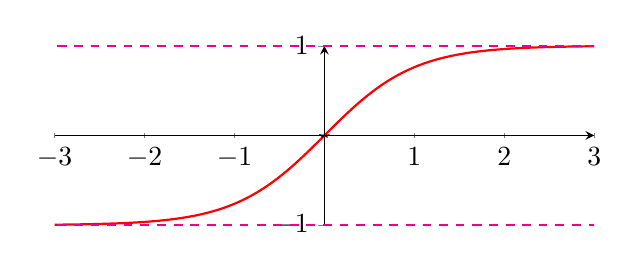
\begin{tikzpicture}
	\begin{axis}[
	samples=1000,
	xscale=1,yscale=0.4,
	xmin=-3,xmax=3,xtick={-3,-2,-1,0,1,2,3},
	ymin=-1,ymax=1,ytick={-1,0,1},
	axis lines=center
	]
	\addplot+[mark=none,color=red,thick] {tanh(x)};
	\addplot+[mark=none,color=magenta,dashed,thick] {1};
	\addplot+[mark=none,color=magenta,dashed,thick] {-1};
	\addplot coordinates {(0,0)};
	\end{axis}
	\end{tikzpicture}
	\subsubsection*{Propriété}
	\begin{enumerate}
		\item Définie et continue sur $\mathbb{R}$
		\item Impaire
		\item Même signe que $\sinh$
		\item Admet une asymptote horizontale en $\pm\infty$ d'équation $y=\pm 1$ (|$\tanh(x)$|$<1$)
		\item Dérivable sur tout $\mathbb{R}$ : \fbox{$\tanh'(x)=1-\tanh^2(x)=\frac{1}{\cosh^2(x)}$}
		\item Admet un point d'inflexion en $(0,0)$
	\end{enumerate}
	\section*{Fonction hyperbolique réciproque}
	\subsection*{Cosinus hyperbolique réciproque}
	\subsubsection*{Définition}
	La fonction cosinus hyperbolique est une bijection de $[1;+\infty[$ vers $[0;+\infty[$, elle admet donc une réciproque appelée \textbf{argument cosinus hyperbolique} aussi écrite 
	\text{\color{blue}arcosh} définie par: 
	\begin{align*}
	\text{arcosh}: [1;+\infty[ &\rightarrow [0;+\infty[ \\
	x \hspace{0.3cm} &\rightarrow y =\text{arcosh}(x) \Leftrightarrow x=\cosh(y)
	\end{align*}
	\subsubsection*{Graphe}
	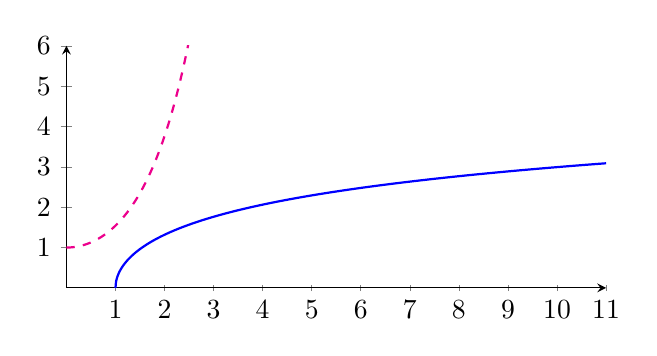
\begin{tikzpicture}
	\begin{axis}[
	samples=1000,
	xscale=1,yscale=0.54,
	xmin=0,xmax=11,xtick={0,1,2,3,4,5,6,7,8,9,10,11},
	ymin=0,ymax=6,ytick={0,1,2,3,4,5,6},
	axis lines=center
	]
	\addplot+[domain=0:2.5,mark=none,color=magenta,thick,dashed] {cosh(x)};
	\addplot+[domain=1:11,mark=none,color=blue,thick] {ln(x+sqrt(x^2-1))};
	\end{axis}
	\end{tikzpicture}
	\subsubsection*{Propriété}
	\begin{enumerate}
		\item Strictement croissante
		\item Admet une écriture logarithmique: arcosh$= \ln(x+\sqrt{x^2-1})$
		\item Est dérivable sur tout son domaine: \fbox{arcosh'$(x)=\frac{1}{\sqrt{x^2-1}}$}
	\end{enumerate}
	\subsection*{Sinus hyperbolique réciproque}
	\subsubsection*{Définition}
	La fonction sinus hyperbolique est une bijection de $\mathbb{R}$ sur $\mathbb{R}$, elle admet donc une réciproque appelée \textbf{argument sinus hyperbolique} aussi écrite 
	\text{\color{green}arsinh} définie par:
	\begin{align*}
	\text{arsinh}: \mathbb{R} &\rightarrow \mathbb{R} \\
	x \hspace{0.3cm} &\rightarrow y =\text{arsinh}(x) \Leftrightarrow x=\sinh(y)
	\end{align*}
	\subsubsection*{Graphe}
	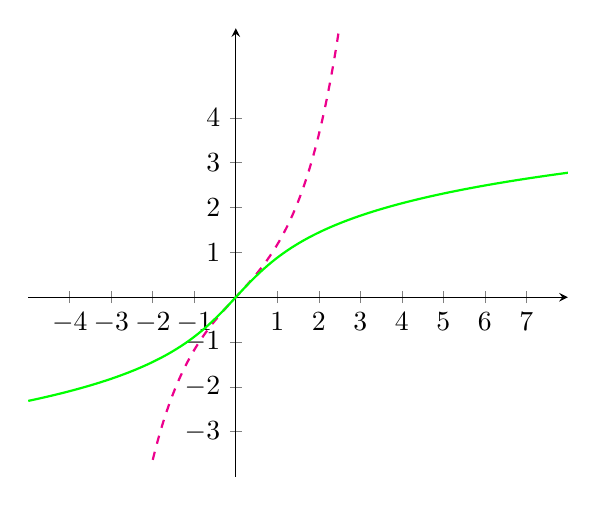
\begin{tikzpicture}
	\begin{axis}[
	samples=1000,
	xscale=1,yscale=1,
	xmin=-5,xmax=8,xtick={-4,-3,-2,-1,0,1,2,3,4,5,6,7},
	ymin=-4,ymax=6,ytick={-3,-2,-1,0,1,2,3,4},
	axis lines=center
	]
	\addplot+[domain=-2:2.7,mark=none,color=magenta,thick,dashed] {sinh(x)};
	\addplot+[domain=-5:9,mark=none,color=green,thick] {ln(x+sqrt(x^2+1))};
	\end{axis}
	\end{tikzpicture}
	\subsubsection*{Propriété}
	\begin{enumerate}
		\item Strictement croissante sur tout $\mathbb{R}$
		\item Possède une écriture logarithmique: arsinh$(x)=\ln(x+\sqrt{x^2+1})$
		\item Est dérivable sur son domaine: \fbox{arsinh'$(x)=\frac{1}{\sqrt{x^2+1}}$}
	\end{enumerate}
	\subsection*{Tangente hyperbolique réciproque}
	\subsubsection*{Définition}
	La fonction tangente hyperbolique est une bijection de $\mathbb{R}$ sur $]-1;1[$, elle admet donc une réciproque appelée \textbf{argument tangente hyperbolique} aussi écrite \text{\color{red}artanh} définie par:
	\begin{align*}
	\text{artanh}: ]-1;1[ &\rightarrow \mathbb{R} \\
	x \hspace{0.3cm} &\rightarrow y =\text{artanh}(x) \Leftrightarrow x=\tanh(y)
	\end{align*}
	\subsubsection*{Graphe}
	\begin{tikzpicture}
	\begin{axis}[
	samples=1000,
	xscale=2,yscale=2,
	xmin=-5,xmax=8,xtick={-4,-3,-2,-1,0,1,2,3,4,5,6,7},
	ymin=-4,ymax=5,ytick={-3,-2,-1,0,1,2,3,4},
	axis lines=center
	]
	\addplot+[domain=-5:8,mark=none,color=magenta,thick,dashed] {tanh(x)};
	\addplot+[domain=-1:1,mark=none,color=red,thick] {(1/2)*ln((1+x)/(1-x))};
	\end{axis}
	\end{tikzpicture}
	\subsubsection*{Propriété}
	\begin{enumerate}
		\item Est strictement croissante sur $]-1;1[$.
		\item Possède une écriture logarithmique: artanh$(x) = \dfrac{1}{2}\ln\left(\dfrac{1+x}{1-x}\right)$
		\item Dérivable sur son domaine: artanh'$(x)=\dfrac{1}{1-x^2}$
	\end{enumerate}
\end{document}